\documentclass[tikz,border=5]{standalone}
\usepackage{amsmath, amsthm, amssymb, amsfonts}
\usepackage{tikz, bbding, tikz-3dplot}
\usetikzlibrary{patterns}
\usetikzlibrary{matrix}
\usetikzlibrary{tikzmark}
\usetikzlibrary{positioning}
\usetikzlibrary{fit}
\usetikzlibrary{shadows.blur}
\usetikzlibrary{shapes.symbols}
\usetikzlibrary{shapes.geometric}
\usetikzlibrary{calc, decorations.pathreplacing}

\begin{document}

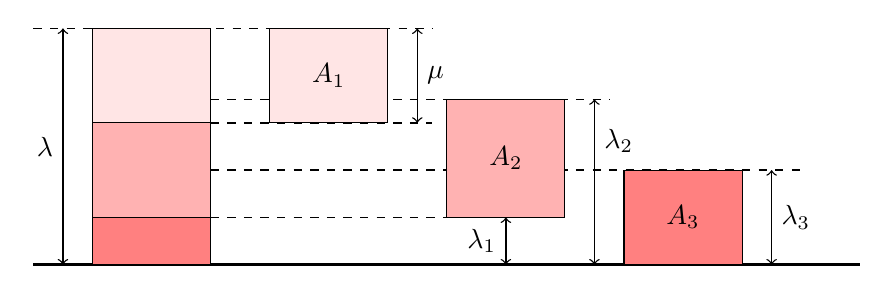
\begin{tikzpicture}[scale=1.5]
			\def \d {0.5}
			\def \w {1}
			\def \h {2}
			
			%Ground and main signal pillar
			\draw [line width = 1] (0,0) -- ({{6*\d+4*\w}},0);
			
			% Markers
			\draw [dashed, line width = 0.5] (0, \h) -- ({2.75*\d+2*\w}, \h);
			\draw [dashed, line width = 0.5] ({\d+\w}, {0.6*\h}) -- ({2.75*\d+2*\w}, {0.6*\h});
			\draw [dashed, line width = 0.5] ({\d+\w}, {0.7*\h}) -- ({3.75*\d+3*\w}, {0.7*\h});
			\draw [dashed, line width = 0.5] ({\d+\w}, {0.2*\h}) -- ({3*\d+2*\w}, {0.2*\h});
			\draw [dashed, line width = 0.5] ({\d+\w}, {0.4*\h}) -- ({5*\d+4*\w}, {0.4*\h});
			
			\draw [<->, line width = 0.5] ({\d/2}, 0) -- ({\d/2}, \h) node [pos = 0.5, left] {$\lambda$};
			\draw [<->, line width = 0.5] ({2.5*\d+2*\w}, {0.6*\h}) -- ({2.5*\d+2*\w}, {\h}) node [pos = 0.5, right] {$\mu$};
			\draw [<->, line width = 0.5] ({3*\d+2.5*\w}, {0*\h}) -- ({3*\d+2.5*\w}, {0.2*\h}) node [pos = 0.5, left] {$\lambda_1$};
			\draw [<->, line width = 0.5] ({3.5*\d+3*\w}, {0*\h}) -- ({3.5*\d+3*\w}, {0.7*\h}) node [pos = 0.75, right] {$\lambda_2$};
			\draw [<->, line width = 0.5] ({4.5*\d + 4*\w}, {0*\h}) -- ({4.5*\d + 4*\w}, {0.4*\h}) node [pos = 0.5, right] {$\lambda_3$};
			
			% Signal pillar
			\draw [fill=red!10] (\d, \h) rectangle ({\d+\w}, {0.6*\h});
			\draw [fill=red!30] (\d, {0.6*\h}) rectangle ({\d+\w}, {0.2*\h});
			\draw [fill=red!50] (\d, {0.2*\h}) rectangle ({\d+\w}, 0);
			
			% Subsections
			\draw [fill = red!10] ({2*\d+\w}, {0.6*\h}) rectangle ({2*\d + 2*\w}, \h) node [pos = 0.5] {$A_1$};
			\draw [fill = red!30] ({3*\d+2*\w}, {0.2*\h}) rectangle ({3*\d + 3*\w}, {0.7*\h}) node [pos = 0.5] {$A_2$};
			\draw [fill = red!50] ({4*\d+3*\w}, {0*\h}) rectangle ({4*\d + 4*\w}, {0.4*\h}) node [pos = 0.5] {$A_3$};
			
		\end{tikzpicture}

\end{document}